\begin{figure*}
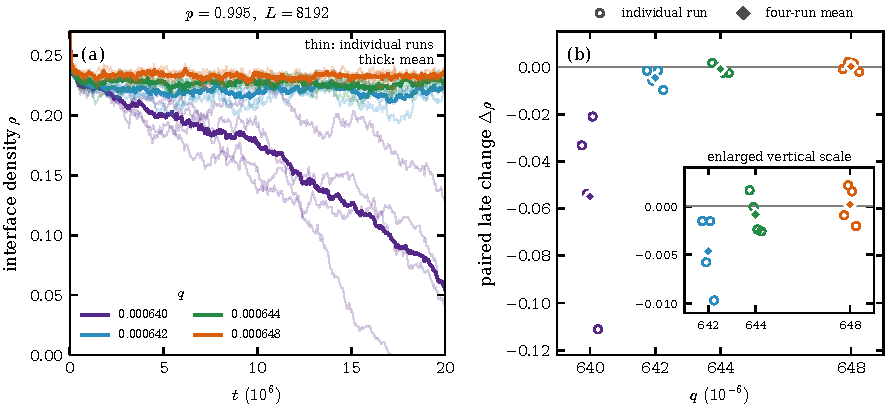
\includegraphics[width=\textwidth]{figs/fig_gpu_near20m}
\caption{Largest-system time dependence near the voter point,
$p=0.995$, $\alpha=1/2$, and $L=8192$. All four declared independent
runs at each $q=0.000640$, 0.000642, 0.000644, and 0.000648 are followed
to $T=2\times10^7$. (a) Thin curves show the individual trajectories
and thick curves their equal-run means. The trajectory that reaches
consensus at $q=0.000640$ contributes its known zero activity thereafter.
(b) Open circles show each run's time-weighted mean density over
$15$--$20\times10^6$ minus that over $10$--$15\times10^6$; diamonds
show the four-run means. Horizontal offsets separate the four runs
visually. The inset repeats the three higher-$q$ groups on an enlarged
vertical scale. The midpoint cohort at $q=0.000642$ was declared
independently after the original grid. The displayed run variation
does not assign a calibrated confidence level or establish stationarity.}
\label{fig:gpu_near20m}
\end{figure*}
